\section{Metodología}

\subsection{Diseño del estudio y fuente de datos}
Se desarrolló un estudio tecnológico y analítico de carácter descriptivo, cuantitativo y auditable sobre el microdato oficial \texttt{data/persona.csv}. El archivo original contiene 39.497 filas y 275 atributos, ocupando 34.568.646 bytes con una huella criptográfica SHA-256 verificada:
\begin{quote}\small\ttfamily
568e82e3039d991a1ee0d8e2056448f8c465c03ffa838330c4f1522dd77bddc8
\end{quote}
Como referencia semántica auxiliar se utilizó el diccionario de datos oficial del INE para el formulario F27 (EH2025\_Persona), estableciendo puentes entre variables sin alterar la fuente original.

\subsection{Etapas del procedimiento operativo}
Siguiendo las fases del ciclo CRISP-DM y KDD, el procedimiento se estructuró en siete etapas reproducibles (ilustradas en la figura \ref{fig:crisp_kdd}):

\begin{enumerate}[leftmargin=0.5in]
  \item \textbf{Comprensión y contrato de datos:} Formalización del esquema de 275 variables, definición de tipos admisibles, clasificación de campos sensibles y estipulación de inmutabilidad sobre el raw.
  \item \textbf{Ingesta e inspección estructural:} Lectura controlada en modo texto para prevenir conversiones automáticas erróneas de ceros o tokens especiales; validación de encabezados únicos y anchura uniforme de registros.
  \item \textbf{Diagnóstico y perfilado multivariado:} Medición de tokens de ausencia (\texttt{""} vs. \texttt{NA} vs. \texttt{0}), cardinalidad de categorías, rangos cuantitativos e identificación de valores extremos mediante IQR.
  \item \textbf{Diseño y aprobación de reglas:} Formulación de reglas respaldadas por teoría física, lingüística o matemática, con condición, acción, universo de impacto y política de rechazo.
  \item \textbf{Preparación y ejecución controlada:} Aplicación secuencial de las reglas autorizadas, generando la versión maestra limpia (\texttt{persona\_clean\_master.parquet}) y registrando toda alteración en bitácora append-only.
  \item \textbf{Modelado por universos y derivación de vistas:} Segmentación de la población en 11 vistas temáticas especializadas basadas estrictamente en los saltos y preguntas filtro de la encuesta.
  \item \textbf{Auditoría, publicación atómica y despliegue:} Verificación censal de dimensiones y claves, persistencia de manifiestos y hashes en JSON local, y sincronización transaccional con la aplicación web Flask.
\end{enumerate}

\begin{figure}[htbp]
\centering
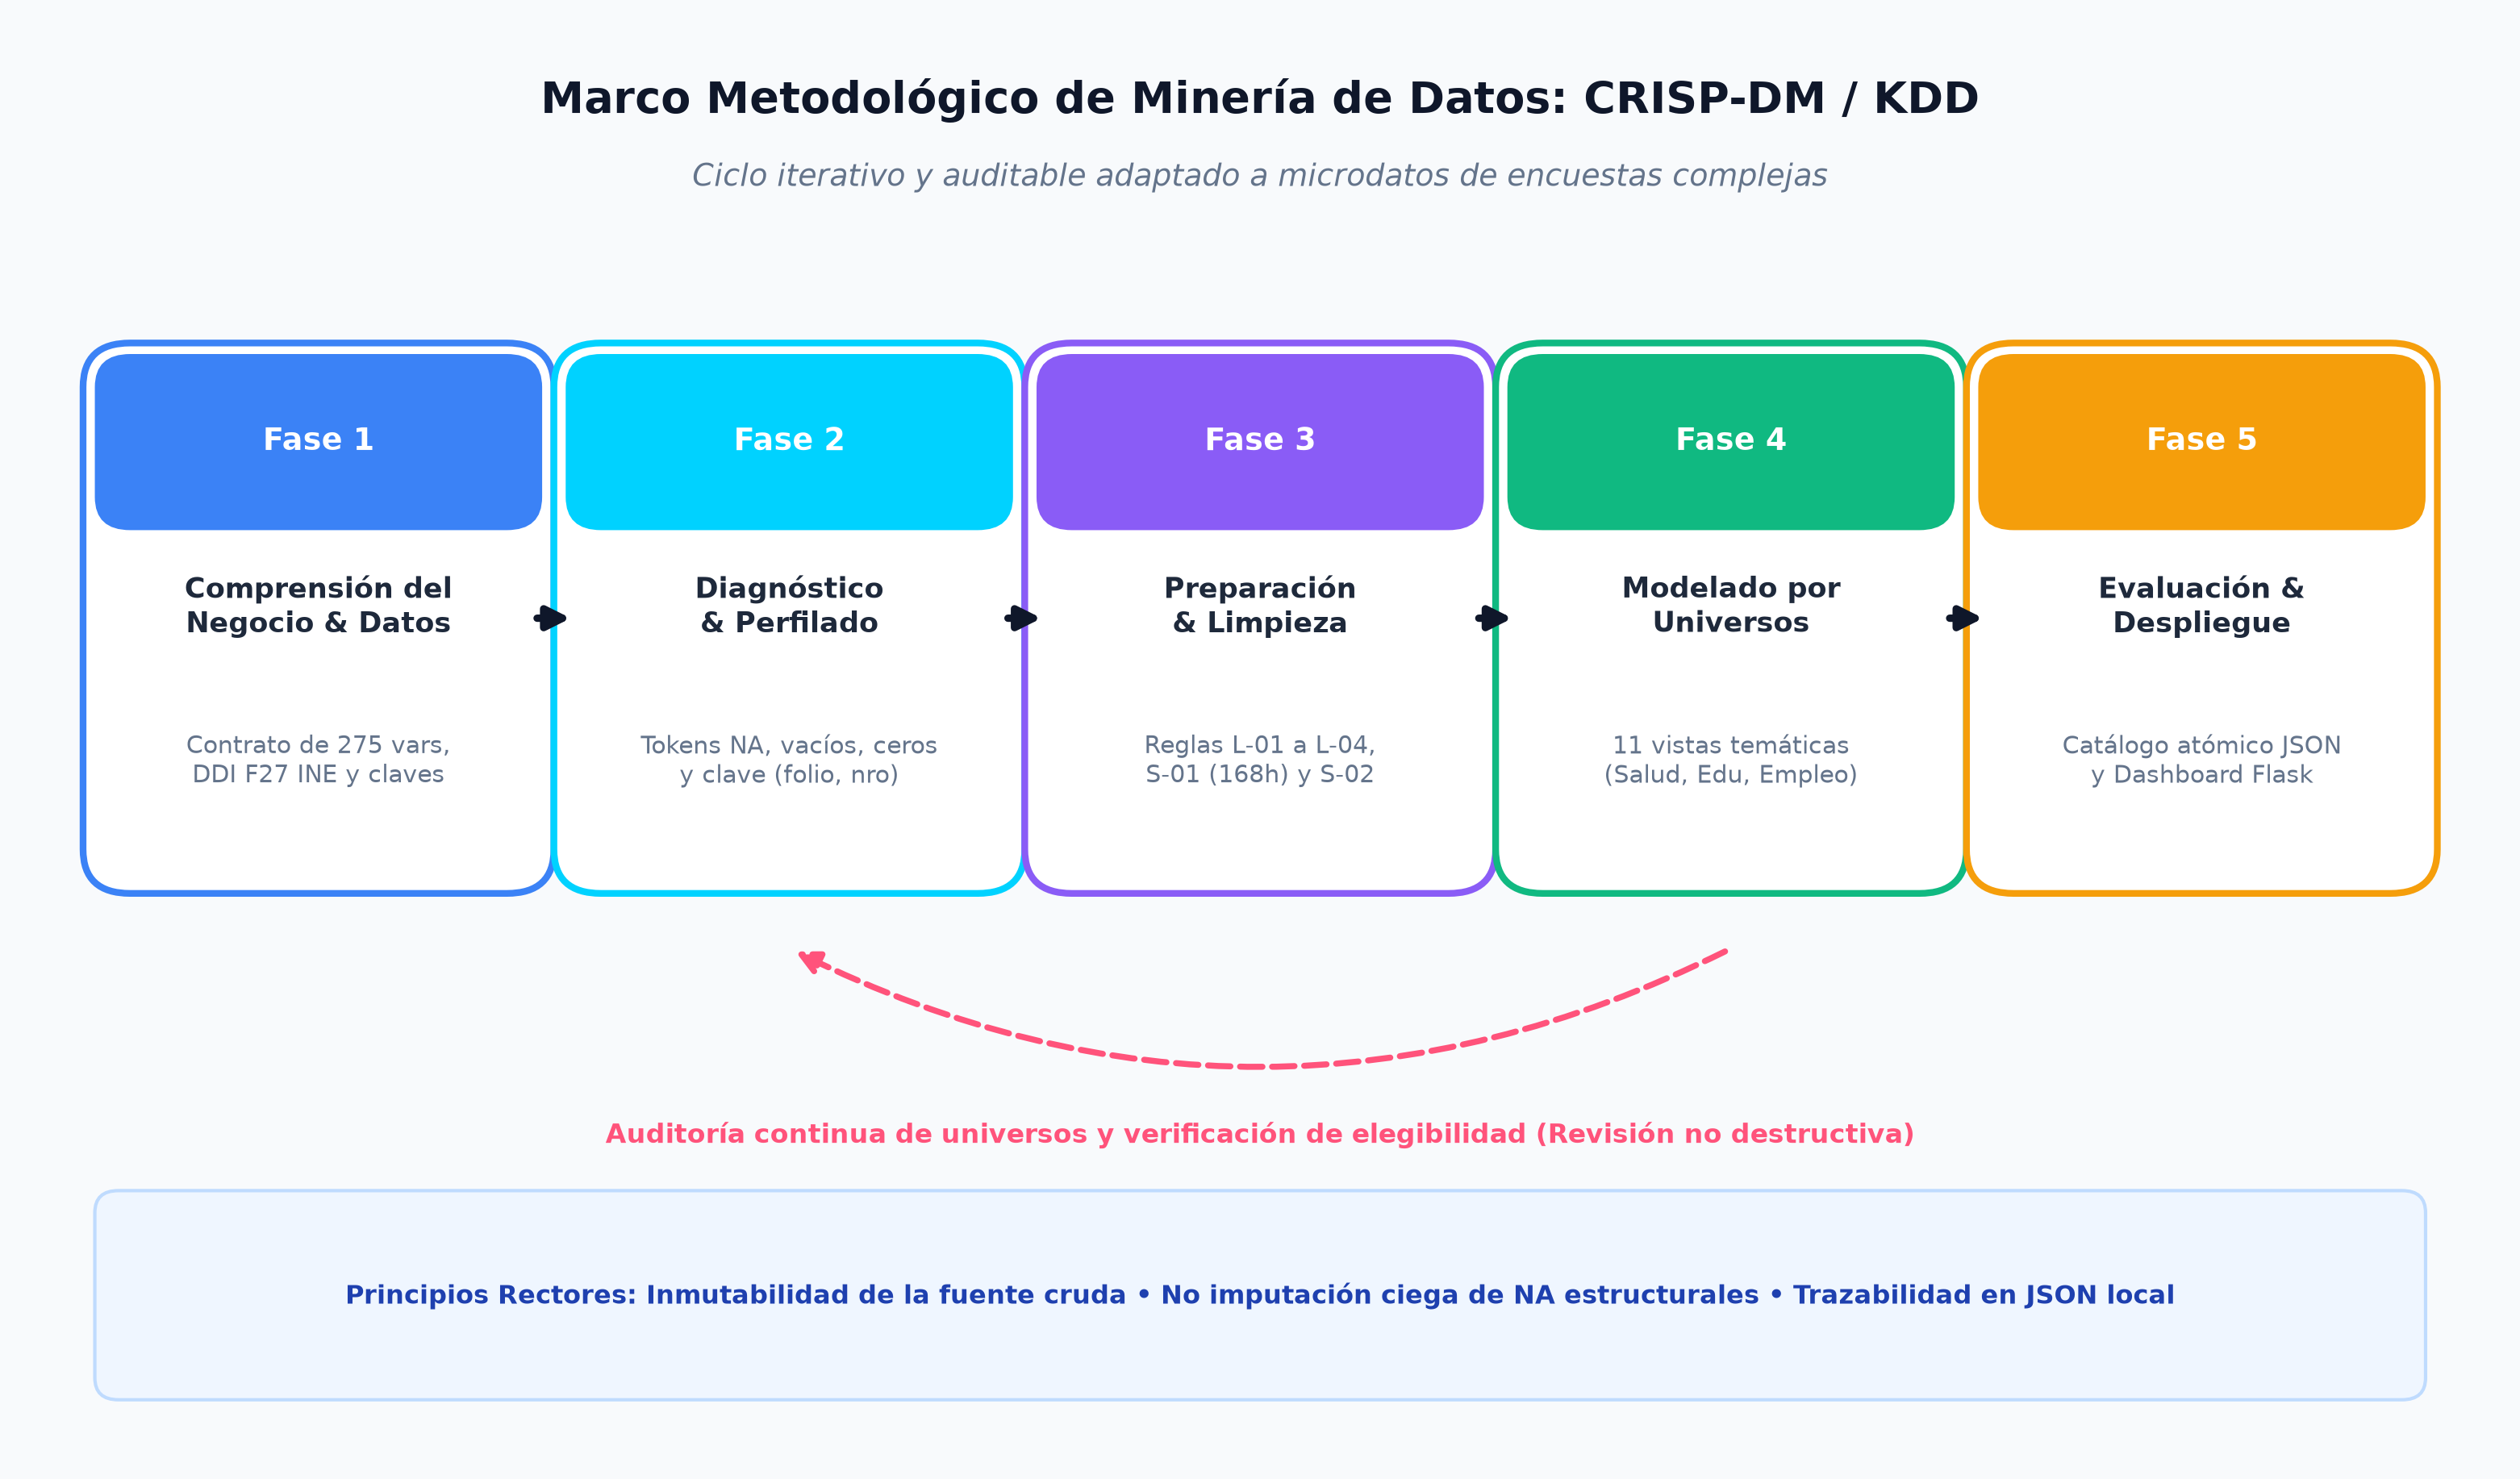
\includegraphics[width=0.98\textwidth]{figuras/fig1_metodologia_crisp_kdd.png}
\caption{Ciclo de vida metodológico CRISP-DM / KDD adaptado al proyecto}
\label{fig:crisp_kdd}
\par\vspace{3pt}\parbox{0.98\textwidth}{\footnotesize\textit{Nota.} Esquema de las cinco fases operativas del proyecto y su bucle iterativo de auditoría de universos. Elaboración propia a partir del marco teórico de Minería de Datos.}
\end{figure}

\begin{figure}[htbp]
\centering
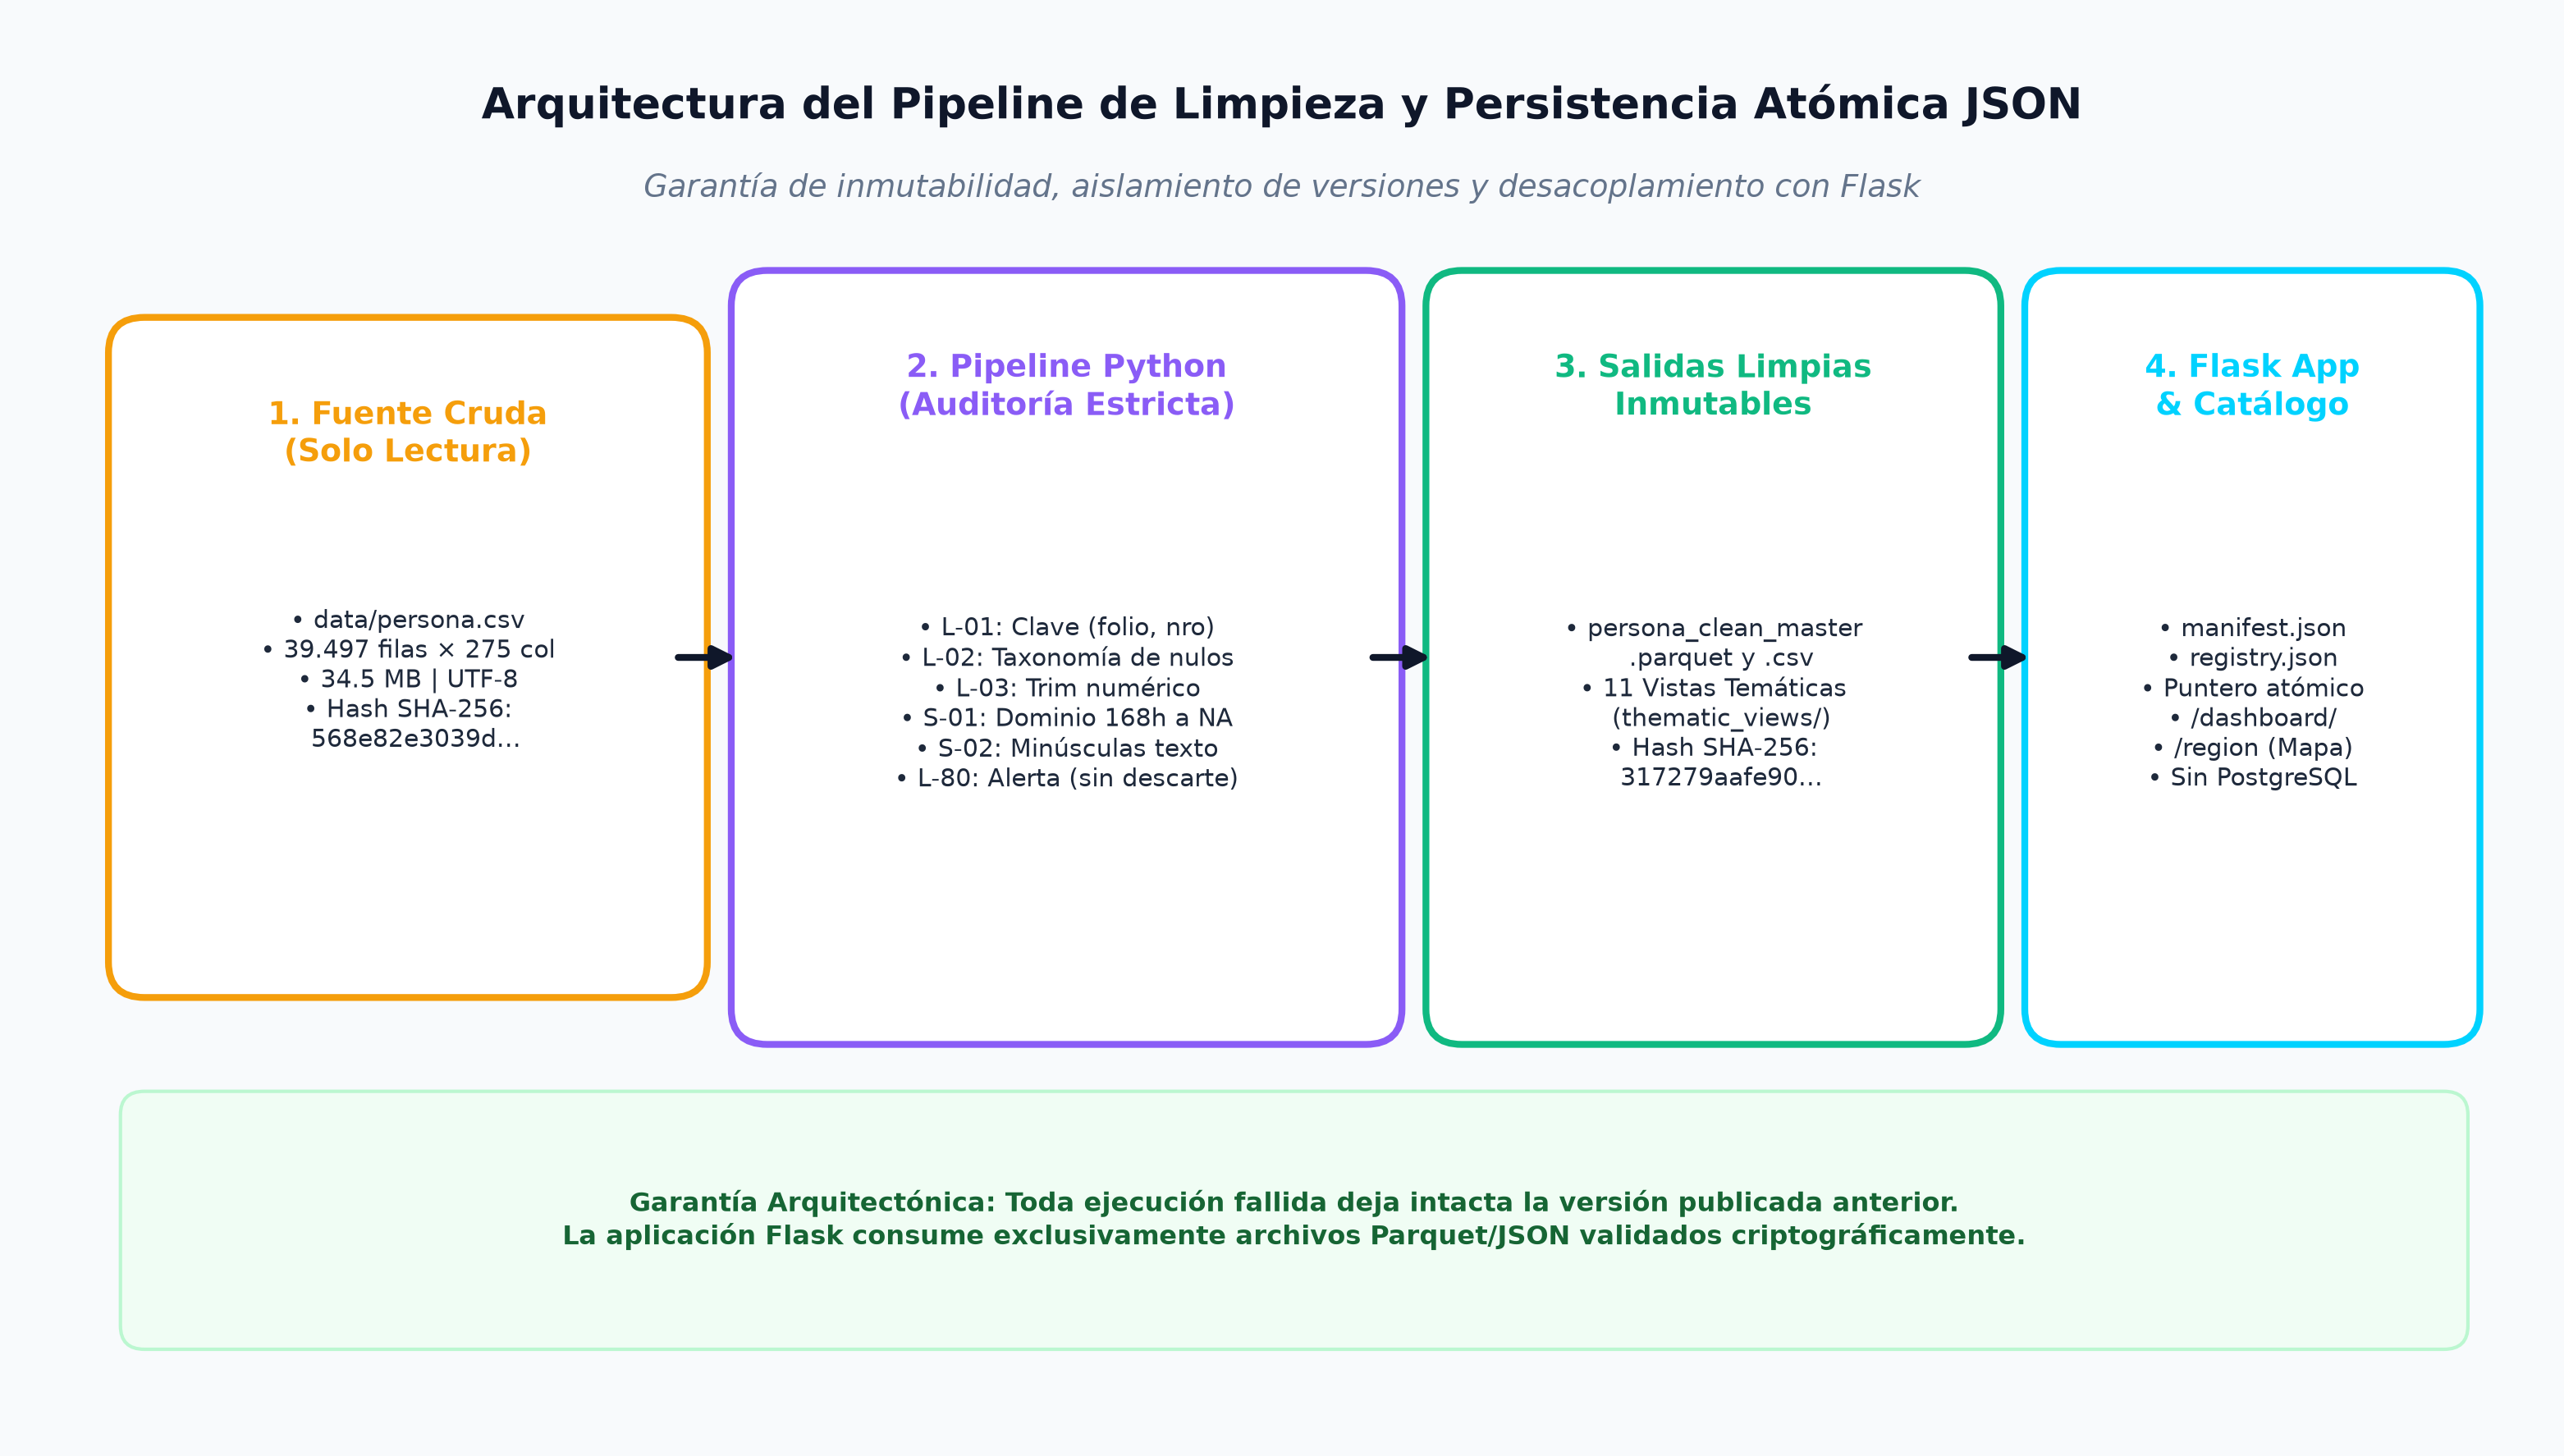
\includegraphics[width=0.98\textwidth]{figuras/fig2_arquitectura_pipeline_json.png}
\caption{Arquitectura del pipeline de limpieza, persistencia atómica JSON y desacoplamiento con Flask}
\label{fig:arquitectura_pipeline}
\par\vspace{3pt}\parbox{0.98\textwidth}{\footnotesize\textit{Nota.} Flujo de transformación que preserva la inmutabilidad de la fuente cruda, materializa el maestro Parquet y actualiza los punteros JSON locales sin gestor relacional externo.}
\end{figure}

\subsection{Catálogo de reglas de limpieza y calidad ejecutadas}
El pipeline ejecuta de manera determinista las siguientes reglas de calidad:

\begin{itemize}[leftmargin=0.5in]
  \item \textbf{Regla L-01 (Clave Primaria Compuesta):} Tipado a enteros positivos y validación estricta de unicidad sobre la tupla relacional \texttt{(folio, nro)}, confirmando que \texttt{folio} identifica la vivienda/hogar y \texttt{nro} al integrante familiar. Se comprobaron 39.497 tuplas únicas (0 duplicados y 0 vacíos).
  \item \textbf{Regla L-02 (Taxonomía de Tokens de Ausencia):} Tratamiento diferenciado de celdas vacías (\texttt{""}), tokens explícitos (\texttt{NA}) y ceros legítimos (\texttt{0}), evitando la colisión o imputación prematura de valores fuera de universo.
  \item \textbf{Regla L-03 (Normalización de Espacios - Trim):} Eliminación de espacios en blanco residuales en las 256 columnas numéricas y códigos categóricos, preservando sin alteración el texto libre.
  \item \textbf{Regla L-04 (Validación de Dominios Categóricos):} Verificación de que variables clave cumplan los códigos oficiales del INE (\texttt{s01a\_01} $\in \{1,2\}$ para sexo, \texttt{depto} $\in \{1..9\}$ y \texttt{area} $\in \{1,2\}$). Cero anomalías detectadas.
  \item \textbf{Regla S-01 (Frontera Física en Horas Semanales):} Validación del límite biológico infranqueable de 168 horas semanales ($7 \times 24$) en variables de jornada laboral (\texttt{phrs}, \texttt{shrs}, \texttt{tothrs}). Tres registros con valores imposibles (171.5h, 180h y 192h) fueron reasignados a \texttt{NA} con registro detallado en bitácora append-only, sin suprimir las filas.
  \item \textbf{Regla S-02 (Normalización Textual Controlada):} Conversión exclusiva a minúsculas en 13 variables de respuesta abierta identificadas como campos de especificación en el diccionario, sin modificar identificadores ni categorías.
  \item \textbf{Regla L-80 (Umbral Técnico Informativo):} Mantiene como advertencia de revisión aquellas variables con más del 80\% de ausencia global, prohibiendo su exclusión destructiva del maestro para no eliminar preguntas condicionales legítimas.
\end{itemize}

\subsection{Estrategia de verificación y control muestral (QA)}
Para validar la no regresión y la integridad de las transformaciones, se implementó una suite automatizada de 16 pruebas sintéticas unitarias que verifican la retención de columnas con 100\% de ausencia, la idempotencia de los algoritmos de trim, el bloqueo preventivo ante claves duplicadas y la lectura protegida por hash SHA-256. Asimismo, se seleccionó una muestra determinista de control de 381 hogares (1.216 personas) estratificada por departamento y área para auditoría intrahogar.
